\chapter{Lista}

Ohjelmoinnin perustietorakenne on taulukko,
joka on mainio tietorakenne, mutta siinä on yksi puute.
Kun luomme taulukon, meidän täytyy antaa sille
kiinteä koko, emmekä voi muuttaa kokoa myöhemmin.
Esimerkiksi seuraava koodi luo taulukon,
jossa on kiinteästi kymmenen alkiota:

\begin{code}
int[] taulu = new int[10];
\end{code}

Tämä on ongelma, koska meillä ei välttämättä ole
taulukon luontihetkellä käsitystä, montako alkiota
haluaisimme tallentaa siihen myöhemmin.

Tämän luvun tavoitteemme on luoda tietorakenne,
joka muistuttaa taulukkoa, mutta sallii alkioiden
lisäämisen ja poistamisen.
Kutsumme tietorakennetta nimellä \emph{lista}.
Tutustumme kahteen tapaan listan toteuttamiseen,
joissa molemmissa on omat hyvät ja huonot puolensa.

\section{Taulukkolista}

\emph{Taulukkolista} on lista, joka on tallennettu taulukkoon.
Esimerkiksi seuraava koodi luo taulukon,
joka vastaa listaa $[3,7,2,5]$:

\begin{code}
int[] lista = {3,7,2,5};
\end{code}

Ongelmana on vain, että taulukon koko on kiinteä,
vaikka haluaisimme pystyä lisäämään ja poistamaan
alkioita.
Löydämme ongelmaan pian ratkaisun, mutta sitä ennen
aiheellinen kysymys on:
miksi ohjelmointikielten suunnittelijat ovat olleet niin keljuja,
että he eivät ole antaneet meille suoraan mahdollisuutta muuttaa
taulukon kokoa?

Tähän on hyvä selitys, joka liittyy siihen,
miten taulukko on tallennettu tietokoneen muistissa.
Tarkastellaan esimerkkinä seuraavaa koodia:

\begin{code}
int[] a = {1,4,2};
int[] b = {5,3,2,5};
\end{code}

\begin{figure}
\center
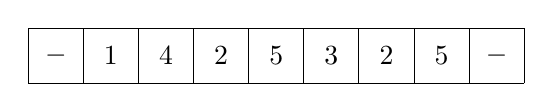
\begin{tikzpicture}[scale=0.7]
\draw (0,0) grid (9,1);
\node at (0.5,0.5) {$-$};
\node at (1.5,0.5) {$1$};
\node at (2.5,0.5) {$4$};
\node at (3.5,0.5) {$2$};
\node at (4.5,0.5) {$5$};
\node at (5.5,0.5) {$3$};
\node at (6.5,0.5) {$2$};
\node at (7.5,0.5) {$5$};
\node at (8.5,0.5) {$-$};
\end{tikzpicture}
\caption{Taulukot $[1,4,2]$ ja $[5,3,2,5]$ tietokoneen muistissa.}
\label{fig:taumui}
\end{figure}

Kuva \ref{fig:taumui} näyttää mahdollisen tavan, miten taulukot
\texttt{a} ja \texttt{b} asettuvat muistissa.
Taulukossa \texttt{a} on kolme alkiota,
joten sille on varattu kolme paikkaa muistista,
ja taulukossa \texttt{b} on neljä alkiota,
joten sille on varattu neljä paikkaa muistista.
Taulukolle varataan aina yhtenäinen muistialue,
minkä ansiosta pääsemme käsiksi sen alkioihin
helposti ajassa $O(1)$.

Kuvassa näkyy ilmeinen syy,
minkä vuoksi emme voi laajentaa taulukon kokoa
luonnin jälkeen:
tyypillisesti muistissa on heti taulukon perässä muuta
tarpeellista tietoa, jota ei saa poistaa.
Jos lisäisimme taulukon \texttt{a} perään uuden alkion,
meidän täytyisi tuhota taulukon \texttt{b} ensimmäinen alkio,
mikä ei tule kysymykseen.
Ainoa tapa laajentaa taulukkoa onkin varata
jostain muualta muistista enemmän tilaa ja kopioida
taulukon sisältö sinne.
Juuri näin joudumme tekemään, kun toteutamme listan taulukkona.

\subsection{Muutokset lopussa}

Toteutamme ensin taulukkolistan, jossa voimme
lisätä ja poistaa alkioita listan lopussa.
Tallennamme listan taulukkona niin,
että tietty määrä alkioita taulukon alussa on listan käytössä
ja loput tyhjät kohdat on varattu tuleville alkioille.
Tämän ansiosta pystymme lisäämään uuden alkion listalle
ajassa $O(1)$, jos taulukossa on tilaa,
koska meidän riittää ottaa käyttöön seuraava
vapaana oleva kohta taulukosta.

Kuva \ref{fig:listau} näyttää esimerkin,
jossa taulukossa on tilaa yhteenä kahdeksalle alkiolle
ja siihen on tallennettu lista $[3,7,2,5]$.
Taulukon neljä ensimmäistä alkiota on siis listan käytössä,
ja muut ovat varalla tulevia alkioita varten.
Kun lisäämme listan loppuun uuden alkion 6,
otamme käyttöön taulukosta uuden kohdan, johon alkio sijoitetaan.

\begin{figure}
\center
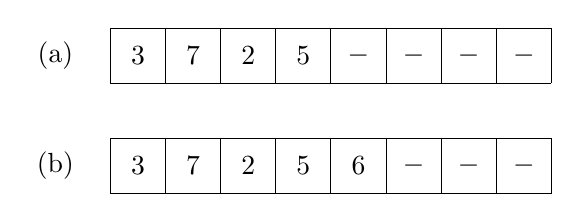
\begin{tikzpicture}[scale=0.7]
\begin{scope}
\draw (0,0) grid (8,1);
\node at (-1,0.5) {(a)};
\node at (0.5,0.5) {$3$};
\node at (1.5,0.5) {$7$};
\node at (2.5,0.5) {$2$};
\node at (3.5,0.5) {$5$};
\node at (4.5,0.5) {$-$};
\node at (5.5,0.5) {$-$};
\node at (6.5,0.5) {$-$};
\node at (7.5,0.5) {$-$};
\end{scope}
\begin{scope}[yshift=-2cm]
\draw (0,0) grid (8,1);
\node at (-1,0.5) {(b)};
\node at (0.5,0.5) {$3$};
\node at (1.5,0.5) {$7$};
\node at (2.5,0.5) {$2$};
\node at (3.5,0.5) {$5$};
\node at (4.5,0.5) {$6$};
\node at (5.5,0.5) {$-$};
\node at (6.5,0.5) {$-$};
\node at (7.5,0.5) {$-$};
\end{scope}
\end{tikzpicture}
\caption{(a) Lista $[3,7,2,5]$ tallennettuna taulukkoon. (b) Listan loppuun lisätään alkio 6.}
\label{fig:listau}
\end{figure}

\begin{figure}
\center
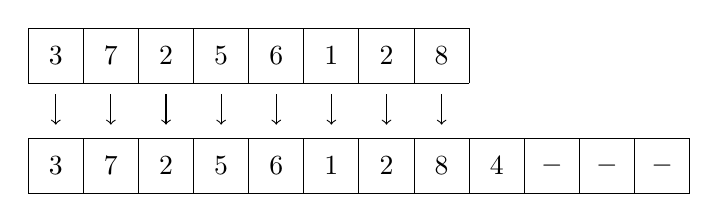
\begin{tikzpicture}[scale=0.7]
\begin{scope}
\draw (0,0) grid (8,1);
\node at (0.5,0.5) {$3$};
\node at (1.5,0.5) {$7$};
\node at (2.5,0.5) {$2$};
\node at (3.5,0.5) {$5$};
\node at (4.5,0.5) {$6$};
\node at (5.5,0.5) {$1$};
\node at (6.5,0.5) {$2$};
\node at (7.5,0.5) {$8$};
\foreach \x in {0,...,7} \draw[->] (\x+0.5,-0.2) -- (\x+0.5,-0.75);
\end{scope}
\begin{scope}[yshift=-2cm]
\draw (0,0) grid (12,1);
\node at (0.5,0.5) {$3$};
\node at (1.5,0.5) {$7$};
\node at (2.5,0.5) {$2$};
\node at (3.5,0.5) {$5$};
\node at (4.5,0.5) {$6$};
\node at (5.5,0.5) {$1$};
\node at (6.5,0.5) {$2$};
\node at (7.5,0.5) {$8$};
\node at (8.5,0.5) {$4$};
\node at (9.5,0.5) {$-$};
\node at (10.5,0.5) {$-$};
\node at (11.5,0.5) {$-$};
\end{scope}
\end{tikzpicture}
\caption{Taulukkoon ei mahdu enää uutta alkiota. Meidän täytyy varata uusi suurempi taulukko
ja kopioida vanhan taulukon sisältö sinne.}
\label{fig:lisuus}
\end{figure}

Mitä tapahtuu sitten, kun jossain vaiheessa koko taulukko
on täynnä eikä uusi listalle lisättävä alkio mahdu enää taulukkoon?
Tällöin meidän täytyy ensin varata uusi suurempi taulukko ja
kopioida kaikki vanhan taulukon alkiot siihen.
Vasta tämän jälkeen voimme lisätä uuden alkion listalle.
Tämä vie aikaa $O(n)$, koska kopioimme kaikki listan alkiot
uuteen paikkaan muistissa.
Esimerkiksi kuvassa \ref{fig:lisuus} uusi alkio 4 ei mahdu taulukkoon,
joten joudumme varaamaan uuden taulukon ja kopioimaan alkiot.

Olemme saaneet siis aikaan listan, jossa lisääminen
vie aikaa \emph{joko} $O(1)$ tai $O(n)$ riippuen siitä,
mahtuuko alkio nykyiseen taulukkoon vai täytyykö
meidän varata uusi taulukko.
Jotta lista olisi käyttökelpoinen, hidas $O(n)$-operaatio
ei saisi esiintyä liian usein.
Osoittautuu, että saavutamme tämän tavoitteen,
kunhan varaamme uuden taulukon aina reilusti aiempaa suuremmaksi.
Tavanomainen ratkaisu on \emph{kaksinkertaistaa} taulukon koko aina,
kun varaamme uuden taulukon.
Kun toimimme näin, jokaisen alkion lisääminen listalle vie
\emph{keskimäärin} vain $O(1)$ aikaa.

Voimme ajatella asian näin: jokainen listalle lisättävä alkio
maksaa \emph{pääsy\-maksuna} kolme euroa.
Tästä yksi euro menee listalle liittymiseen ja kaksi euroa jäävät säästöön.
Sitten kun aikanaan listalle täytyy varata suurempi taulukko,
jokainen viime erässä lisätty alkio maksaa yhden euron omasta siirrostaan
ja yhden euron aiemmin lisätyn alkion siirrosta.
Koska taulukon koko kaksinkertaistuu joka vaiheessa,
kolmen euron kiinteä pääsymaksu riittää siihen, että kaikki tulevat
siirrot saadaan kustannettua.

\begin{figure}
\center
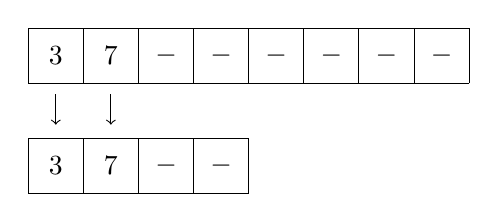
\begin{tikzpicture}[scale=0.7]
\begin{scope}
\draw (0,0) grid (8,1);
\node at (0.5,0.5) {$3$};
\node at (1.5,0.5) {$7$};
\node at (2.5,0.5) {$-$};
\node at (3.5,0.5) {$-$};
\node at (4.5,0.5) {$-$};
\node at (5.5,0.5) {$-$};
\node at (6.5,0.5) {$-$};
\node at (7.5,0.5) {$-$};
\foreach \x in {0,...,1} \draw[->] (\x+0.5,-0.2) -- (\x+0.5,-0.75);
\end{scope}
\begin{scope}[yshift=-2cm]
\draw (0,0) grid (4,1);
\node at (0.5,0.5) {$3$};
\node at (1.5,0.5) {$7$};
\node at (2.5,0.5) {$-$};
\node at (3.5,0.5) {$-$};
\end{scope}
\end{tikzpicture}
\caption{Poistojen jälkeen taulukon koko on käynyt tarpeettoman suureksi,
ja puolitamme taulukon koon.}                                                                        
\label{fig:lispoi}
\end{figure}

Voimme poistaa alkion listan lopusta aina $O(1)$-ajassa,
koska taulukon kokoa ei tarvitse koskaan suurentaa.
Tässä voi kuitenkin tulla ongelmaksi, että monien poistojen
jälkeen taulukossa on turhan paljon tyhjää tilaa lopussa.
Voimme soveltaa tässä käänteisesti samaa ideaa kuin lisäämisessä:
jos poistamisen jälkeen vain \emph{neljännes} taulukosta on käytössä,
puolitamme taulukon koon.
Kuva \ref{fig:lispoi} näyttää esimerkin tällaisesta tilanteesta.
Tällä tavalla poistamiset vievät keskimäärin aikaa $O(1)$.

Miksi sitten emme voisi varata heti aluksi niin suurta taulukkoa,
että lopullinen lista mahtuisi siihen varmasti?
Tässä olisi huonona puolena, että listamme tuhlaisi paljon muistia.
Ohjelmassa saattaa olla samaan aikaan käytössä monia listoja,
ja haluamme, että listalle varattu taulukko on samaa kokoluokkaa
kuin listan todellinen sisältö.

\subsection{Muutokset alussa ja lopussa}

Melko samaan tapaan voimme myös luoda taulukkolistan,
joka sallii tehokkaat alkioiden lisäykset ja poistot
sekä listan alussa että lopussa.
Jotta tämä onnistuisi, muutamme listan tallennustapaa niin,
että lista voi alkaa ja päättyä missä tahansa taulukon
kohdassa ja listan sisältö voi jatkua taulukon lopusta alkuun.
Tämän ansiosta pystymme tekemään lisäyksiä ja poistoja
listan molemmissa päissä.

\begin{figure}
\center
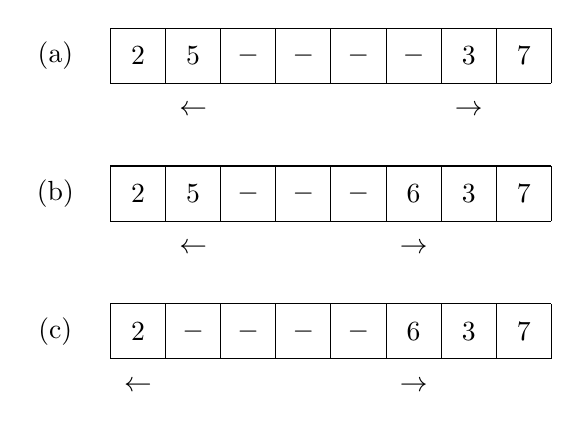
\begin{tikzpicture}[scale=0.7]
\begin{scope}
\draw (0,0) grid (8,1);
\node at (-1,0.5) {(a)};
\node at (0.5,0.5) {$2$};
\node at (1.5,0.5) {$5$};
\node at (2.5,0.5) {$-$};
\node at (3.5,0.5) {$-$};
\node at (4.5,0.5) {$-$};
\node at (5.5,0.5) {$-$};
\node at (6.5,0.5) {$3$};
\node at (7.5,0.5) {$7$};
\node at (1.5,-0.5) {$\leftarrow$};
\node at (6.5,-0.5) {$\rightarrow$};
\end{scope}
\begin{scope}[yshift=-2.5cm]
\draw (0,0) grid (8,1);
\node at (-1,0.5) {(b)};
\node at (0.5,0.5) {$2$};
\node at (1.5,0.5) {$5$};
\node at (2.5,0.5) {$-$};
\node at (3.5,0.5) {$-$};
\node at (4.5,0.5) {$-$};
\node at (5.5,0.5) {$6$};
\node at (6.5,0.5) {$3$};
\node at (7.5,0.5) {$7$};
\node at (1.5,-0.5) {$\leftarrow$};
\node at (5.5,-0.5) {$\rightarrow$};
\end{scope}
\begin{scope}[yshift=-5cm]
\draw (0,0) grid (8,1);
\node at (-1,0.5) {(c)};
\node at (0.5,0.5) {$2$};
\node at (1.5,0.5) {$-$};
\node at (2.5,0.5) {$-$};
\node at (3.5,0.5) {$-$};
\node at (4.5,0.5) {$-$};
\node at (5.5,0.5) {$6$};
\node at (6.5,0.5) {$3$};
\node at (7.5,0.5) {$7$};
\node at (0.5,-0.5) {$\leftarrow$};
\node at (5.5,-0.5) {$\rightarrow$};
\end{scope}
\end{tikzpicture}
\caption{(a) Lista $[3,7,2,5]$ tallennettuna taulukkoon.
(b) Listan alkuun lisätään alkio 6.
(c) Listan lopusta poistetaan alkio 5.}
\label{fig:lismol}
\end{figure}

Kuva \ref{fig:lismol} näyttää esimerkin listan $[3,7,2,5]$
uudesta tallennustavasta.
Merkki $\rightarrow$ osoittaa kohdan, josta lista alkaa,
ja merkki $\leftarrow$ osoittaa kohdan, johon lista päättyy.
Kun haluamme lisätä alkion listan alkuun,
siirrymme vasemmalle kohdasta $\rightarrow$,
ja kun haluamme lisätä alkion listan loppuun,
siirrymme oikealle kohdasta $\leftarrow$.
Kun haluamme poistaa alkioita listasta,
menettelemme käänteisesti.

\begin{figure}
\center
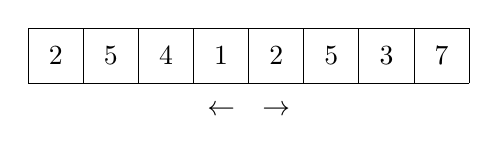
\begin{tikzpicture}[scale=0.7]
\begin{scope}
\draw (0,0) grid (8,1);
\node at (0.5,0.5) {$2$};
\node at (1.5,0.5) {$5$};
\node at (2.5,0.5) {$4$};
\node at (3.5,0.5) {$1$};
\node at (4.5,0.5) {$2$};
\node at (5.5,0.5) {$5$};
\node at (6.5,0.5) {$3$};
\node at (7.5,0.5) {$7$};
\node at (3.5,-0.5) {$\leftarrow$};
\node at (4.5,-0.5) {$\rightarrow$};
\end{scope}
\end{tikzpicture}
\caption{Lista $[2,5,3,7,2,5,4,1]$ täyttää koko taulukon, emmekä voi lisätä uutta alkiota.
Ratkaisuna on varata suurempi taulukko.}
\label{fig:lismol2}
\end{figure}

Jos kohdat $\rightarrow$ ja $\leftarrow$ ovat vierekkäin,
taulukko on täynnä, emmekä voi enää lisätä uutta alkiota
listan alkuun tai loppuun.
Kuva \ref{fig:lismol2} näyttää esimerkin tällaisesta tilanteesta.
Tällöin meidän täytyy varata uusi suurempi taulukko,
johon listan sisältö siirretään.
Voimme menetellä samalla tavalla kuin aiemmin ja
kaksinkertaistaa taulukon koon joka vaiheessa,
jolloin operaatiot vievät keskimäärin aikaa $O(1)$.

\section{Linkitetty lista}

\emph{Linkitetty lista} muodostuu solmuista, joista jokainen sisältää
yhden listan alkion.
Yhteen suuntaan linkitetyssä listassa jokaisessa
solmussa on viittaus listan seuraavaan solmuun.
Kahteen suuntaan linkitetyssä listassa taas
solmut viittaavat sekä listan seuraavaan että edelliseen solmuun.
Viittausten avulla pystymme liikkumaan listassa.

\begin{figure}
\center
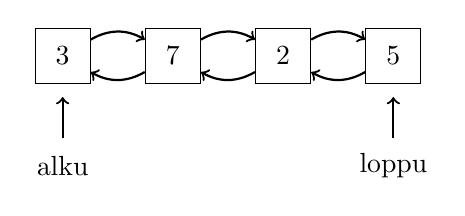
\begin{tikzpicture}[scale=0.7]
\begin{scope}
\node[draw, rectangle, minimum size=7mm] (1) at (0,0) {$3$};
\node[draw, rectangle, minimum size=7mm] (2) at (2,0) {$7$};
\node[draw, rectangle, minimum size=7mm] (3) at (4,0) {$2$};
\node[draw, rectangle, minimum size=7mm] (4) at (6,0) {$5$};
\path[draw,thick,->] (1) edge [bend left] (2);
\path[draw,thick,->] (2) edge [bend left] (3);
\path[draw,thick,->] (3) edge [bend left] (4);
\path[draw,thick,->] (4) edge [bend left] (3);
\path[draw,thick,->] (3) edge [bend left] (2);
\path[draw,thick,->] (2) edge [bend left] (1);
\node at (0,-2) {alku};
\node at (6,-2) {loppu};
\path[draw,thick,->] (0,-1.5) -- (0,-0.75);
\path[draw,thick,->] (6,-1.5) -- (6,-0.75);
\end{scope}
\end{tikzpicture}
\caption{Kahteen suuntaan linkitetty lista, joka sisältää alkiot $[3,7,2,5]$.}
\label{fig:linlis}
\end{figure}

Kuvassa \ref{fig:linlis} on esimerkkinä kahteen suuntaan linkitetty lista,
joka sisältää alkiot $[3,7,2,5]$.
Jokainen alkio viittaa seuraavaan ja edelliseen alkioon,
minkä ansiosta pystymme liikkumaan listassa.
Lisäksi tiedossamme on viittaukset listan alkuun ja loppuun.
Voimme esimerkiksi käydä listan läpi aloittamalla alusta
ja siirtymällä aina seuraavaan solmuun askel kerrallaan.

Kaksisuuntainen linkitys on käytännössä järkevä tapa toteuttaa
linkitetty lista, ja oletamme jatkossa, että listamme on
kahteen suuntaan linkitetty ja meillä on tiedossa viittaukset
listan alkuun ja loppuun.

\subsection{Linkitetyt rakenteet}

Jokaisessa ohjelmointikielessä on omat keinonsa
linkitetyn rakenteen toteuttamiseen.
Javassa voimme toteuttaa linkitetyn rakenteen niin,
että jokainen solmu on oma olionsa.
Esimerkiksi voimme toteuttaa seuraavan luokan \texttt{Solmu},
jonka oliot toimivat linkitetyn listan solmuina:

\begin{code}
public class Solmu {
    public int arvo;
    public Solmu seuraava;
    public Solmu edellinen;

    public Solmu(int arvo, Solmu seuraava, Solmu edellinen) {
        this.arvo = arvo;
        this.seuraava = seuraava;
        this.edellinen = edellinen;
    }
}
\end{code}

Tässä kenttä \texttt{arvo} kertoo solmun arvon,
kenttä \texttt{seuraava} osoittaa seuraavaan solmuun
ja kenttä \texttt{edellinen} osoittaa edelliseen solmuun.
Jos seuraavaa tai edellistä solmua ei ole,
viittauksen tilalla on arvo \texttt{null}.
Tämän luokan avulla voisimme luoda linkitetyn listan $[3,7,2,5]$
seuraavasti:

\begin{code}
Solmu s1, s2, s3, s4;
s1 = new Solmu(3, s2, null);
s2 = new Solmu(7, s3, s1);
s3 = new Solmu(2, s4, s2);
s4 = new Solmu(5, null, s3);
\end{code}

Tämän jälkeen voisimme käydä listan läpi näin alusta loppuun:

\begin{code}
Solmu s = s1;
while (s != null) {
    System.out.println(s.arvo);
    s = s.seuraava;
}
\end{code}

Koodin tulostus on seuraava:

\begin{code}
3
7
2
5
\end{code}

\subsection{Listan operaatiot}

Linkitetyn listan etuna on,
että voimme lisätä ja poistaa
alkioita $O(1)$-ajassa kaikissa listan kohdissa.
Kun haluamme lisätä listalle alkion,
luomme ensin uuden solmun ja muutamme sitten
sen vieressä olevien solmujen viittauksia niin,
että ne viittaavat uuteen solmuun.
Vastaavasti kun haluamme poistaa alkion,
muutamme viittauksia niin, että solmu ohitetaan.

\begin{figure}
\center
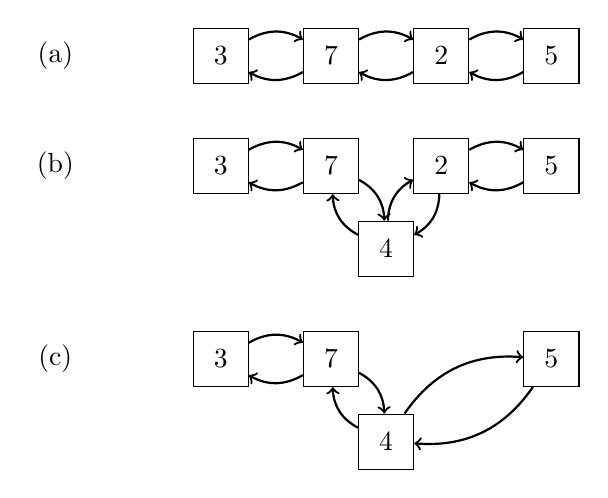
\begin{tikzpicture}[scale=0.7]
\begin{scope}
\node at (-3,0) {(a)};
\node[draw, rectangle, minimum size=7mm] (1) at (0,0) {$3$};
\node[draw, rectangle, minimum size=7mm] (2) at (2,0) {$7$};
\node[draw, rectangle, minimum size=7mm] (3) at (4,0) {$2$};
\node[draw, rectangle, minimum size=7mm] (4) at (6,0) {$5$};
\path[draw,thick,->] (1) edge [bend left] (2);
\path[draw,thick,->] (2) edge [bend left] (3);
\path[draw,thick,->] (3) edge [bend left] (4);
\path[draw,thick,->] (4) edge [bend left] (3);
\path[draw,thick,->] (3) edge [bend left] (2);
\path[draw,thick,->] (2) edge [bend left] (1);
\end{scope}
\begin{scope}[yshift=-2cm]
\node at (-3,0) {(b)};
\node[draw, rectangle, minimum size=7mm] (1) at (0,0) {$3$};
\node[draw, rectangle, minimum size=7mm] (2) at (2,0) {$7$};
\node[draw, rectangle, minimum size=7mm] (3) at (4,0) {$2$};
\node[draw, rectangle, minimum size=7mm] (4) at (6,0) {$5$};
\node[draw, rectangle, minimum size=7mm] (5) at (3,-1.5) {$4$};
\path[draw,thick,->] (1) edge [bend left] (2);
\path[draw,thick,->] (2) edge [bend left] (5);
\path[draw,thick,->] (5) edge [bend left] (3);
\path[draw,thick,->] (3) edge [bend left] (4);
\path[draw,thick,->] (4) edge [bend left] (3);
\path[draw,thick,->] (3) edge [bend left] (5);
\path[draw,thick,->] (5) edge [bend left] (2);
\path[draw,thick,->] (2) edge [bend left] (1);
\end{scope}
\begin{scope}[yshift=-5.5cm]
\node at (-3,0) {(c)};
\node[draw, rectangle, minimum size=7mm] (1) at (0,0) {$3$};
\node[draw, rectangle, minimum size=7mm] (2) at (2,0) {$7$};
\node[draw, rectangle, minimum size=7mm] (4) at (6,0) {$5$};
\node[draw, rectangle, minimum size=7mm] (5) at (3,-1.5) {$4$};
\path[draw,thick,->] (1) edge [bend left] (2);
\path[draw,thick,->] (2) edge [bend left] (5);
\path[draw,thick,->] (5) edge [bend left] (4);
\path[draw,thick,->] (4) edge [bend left] (5);
\path[draw,thick,->] (5) edge [bend left] (2);
\path[draw,thick,->] (2) edge [bend left] (1);
\end{scope}
\end{tikzpicture}
\caption{(a) Alkuperäinen lista $[3,7,2,5]$.
(b) Listan keskelle lisätään alkio $4$.
(c) Listasta poistetaan alkio $2$.}
\label{fig:lismuu}
\end{figure}

Kuva \ref{fig:lismuu} näyttää esimerkin linkitetyn listan käsittelystä.
Listan sisältönä on aluksi $[3,7,2,5]$.
Sitten lisämme listan keskelle alkion 4,
jolloin luomme ensin uuden solmun alkiolle ja muutamme
sitten viittauksia alkioiden 7 ja 2 välillä niin,
että alkio 4 tulee niiden väliin.
Lopuksi poistamme listasta alkion 2, jolloin yhdistämme
alkiot 4 ja 5 suoraan toisiinsa.

Koska meillä on muistissa viittaukset listan alkuun ja loppuun,
pääsemme niihin solmuihin tehokkaasti.
Sen sijaan jos haluamme päästä johonkin muuhun listan kohtaan,
meidän tulee aloittaa alusta tai lopusta ja kulkea askel
kerrallaan viittauksia seuraten.
Niinpä tiettyyn listan kohtaan pääseminen vie aikaa $O(n)$.
Joudumme tekemään näin, koska listan alkiot ovat muistissa
sekalaisissa kohdissa eikä meillä ole suoraa keinoa päästä niihin.

\subsection{Listojen vertailua}

\begin{table}
\center
\begin{tabular}{lrr}
operaatio & taulukkolista & linkitetty lista \\
\hline
pääsy listan alkuun & $O(1)$ & $O(1)$ \\
pääsy listan loppuun & $O(1)$ & $O(1)$ \\ 
pääsy listan keskelle &  $O(1)$ & $O(n)$ \\
lisäys/poisto listan alussa & $O(1)^*$ & $O(1)$ \\
lisäys/poisto listan lopussa & $O(1)^*$ & $O(1)$ \\ 
lisäys/poisto listan keskellä &  $O(n)$ & $O(1)$ \\
\end{tabular}
\caption{Taulukkolistan ja linkitetyn listan operaatioiden
aikavaativuuksia. Merkintä $^*$ tarkoittaa keskimääräistä aikavaativuutta.}
\label{tab:taulin}
\end{table}

Taulukko \ref{tab:taulin} esittää yhteenvedon taulukkolistan ja
linkitetyn listan ominaisuuksista.
Kummassakin toteutuksessa on yksi operaatio,
joka ei ole tehokas.
Taulukkolistassa pääsemme tehokkaasti mihin tahansa listan
kohtaan, mutta on hidasta muokata listaa keskeltä.
Linkitetyssä listassa voimme muokata listaa mistä tahansa,
mutta keskelle pääseminen on hidasta.

Huomaa, että keskelle pääsemisen hitaus rajoittaa melko paljon
linkitetyn listan käyttämistä.
Vaikka pystymme sinänsä muokkaamaan listaa mistä tahansa kohdasta
tehokkaasti, meidän tulee ensin \emph{päästä} kyseiseen kohtaan.
Jos meillä on jostain syystä etukäteen tiedossa viittaus listan keskelle,
voimme muokata kyseistä kohtaa tehokkaasti,
mutta muuten meidän tulee ensin kulkea haluttuun kohtaan,
missä kuluu aikaa $O(n)$.

\section{Javan toteutukset}

Javan standardikirjastossa on monia listojen toteutuksia,
jotka pohjautuvat taulukkolistaan tai linkitettyyn listaan.
Seuraavaksi tutustumme rakenteisiin, joista on usein
hyötyä algoritmien toteutuksessa.

\subsection{\texttt{ArrayList}-rakenne}

\texttt{ArrayList}-rakenne on taulukkolista,
joka sallii tehokkaat lisäykset ja poistot listan lopussa.
Esimerkiksi seuraava koodi luo listan, lisää siihen alkiot
1, 2 ja 3 ja tulostaa listan sisällön.

\begin{code}
ArrayList<Integer> lista = new ArrayList<>();
lista.add(1);
lista.add(2);
lista.add(3);
System.out.println(lista); // [1, 2, 3]
\end{code}

Metodi \texttt{add} toimii keskimäärin ajassa $O(1)$,
joten voimme lisätä tehokkaasti alkioita listan loppuun.

Koska lista on tallennettu taulukkona,
pääsemme myös tehokkaasti käsiksi sen alkioihin
kohdan perusteella.
Metodi \texttt{get} hakee tietyssä kohdassa olevan arvon,
ja metodi \texttt{set} muuttaa arvoa.
Esimerkiksi seuraava koodi tulostaa ensin
listan kohdassa 1 olevan alkion ja muuttaa sitten
sen arvoksi 5.

\begin{code}
System.out.println(lista.get(1)); // 2
lista.set(1,5);
System.out.println(lista.get(1)); // 5
\end{code}

Luokassa \texttt{Collections} on hyödyllisiä metodeita
listan käsittelyyn.
Seuraava koodi järjestää ensin listan,
muuttaa sitten sen järjestyksen käänteiseksi
ja sekoittaa lopuksi järjestyksen.

\begin{code}
Collections.sort(lista);
Collections.reverse(lista);
Collections.shuffle(lista);
\end{code}

\subsection{\texttt{ArrayDeque}-rakenne}

\texttt{ArrayDeque}-rakenne on taulukkolista,
joka sallii tehokkaat lisäykset ja poistot
sekä listan alussa että lopussa.
Alkioita voi lisätä
metodeilla \texttt{addFirst} ja \texttt{addLast}
ja poistaa
metodeilla \texttt{removeFirst} ja \texttt{removeLast}.

\begin{code}
ArrayDeque<Integer> lista = new ArrayDeque<>();
lista.addLast(1);
lista.addFirst(2);
lista.addLast(3);
System.out.println(lista); // [2, 1, 3]
lista.removeFirst();
System.out.println(lista); // [1, 3]
\end{code}

Lisäksi voimme hakea listan ensimmäisen ja viimeisen
alkion metodeilla \texttt{getFirst} ja \texttt{getLast}.

\begin{code}
ArrayDeque<Integer> lista = new ArrayDeque<>();
lista.addLast(1);
lista.addLast(2);
lista.addLast(3);
System.out.println(lista.getFirst()); // 1
System.out.println(lista.getLast()); // 3
\end{code}

Kaikki nämä metodit toimivat keskimäärin ajassa $O(1)$.
Rajoituksena on kuitenkin, että emme pääse käsiksi
listan keskellä oleviin alkioihin, vaan voimme käsitellä
vain listan alkua ja loppua.

\subsection{\texttt{LinkedList}-rakenne}

\texttt{LinkedList}-rakenne toteuttaa kaksisuuntaisen
linkitetyn listan, jossa voimme helposti lisätä ja poistaa
alkioita listan alussa ja lopussa.
Seuraava koodi esittelee asiaa:

\begin{code}
LinkedList<Integer> lista = new LinkedList<>();
lista.addLast(1);
lista.addFirst(2);
lista.addLast(3);
System.out.println(lista); // [2, 1, 3]
lista.removeFirst();
System.out.println(lista); // [1, 3]
\end{code}

Jos haluamme tehdä lisäyksiä ja poistoja muualla listassa,
meidän täytyy ottaa käyttöön \emph{iteraattori}, joka osoittaa haluttuun kohtaan.
Seuraava koodi luo iteraattorin, joka osoittaa ensin listan alkuun.
Sitten siirrämme iteraattoria kaksi askelta eteenpäin ja
lisäämme alkion 5 iteraattorin kohdalle eli listan
toisen ja kolmannen alkion väliin.

\begin{code}
ListIterator<Integer> x = lista.listIterator(0);
x.next();
x.next();
x.add(5);
\end{code}

\texttt{LinkedList} tarjoaa myös metodit
\texttt{get} ja \texttt{set}, joiden avulla
pääsemme käsiksi tietyssä kohdassa listalla olevaan alkioon.
Nämä metodit vievät kuitenkin aikaa $O(n)$,
koska joudumme kulkemaan ensin oikeaan kohtaan listan
alusta tai lopusta.
Tämän vuoksi \texttt{LinkedList} ei ole hyvä valinta,
jos haluamme käsitellä alkioita kohdan perusteella.

\section{Tehokkuusvertailu}

Tärkeä kysymys on, miten tehokkaita taulukkolista ja
linkitetty lista ovat \emph{käytännössä} ja kumpaa meidän
kannattaa käyttää, jos voimme valita.
Seuraavaksi vertailemme Javan taulukkolistan
(\texttt{ArrayList}) ja linkitetyn listan (\texttt{LinkedList})
käytännön tehokkuutta.

Testissä muodostamme ensin taulukon, joka sisältää luvut $1,2,\dots,n$
satunnaisessa järjestyksessä.
Tämän jälkeen luomme tyhjän listan ja käymme taulukon läpi
vasemmalta oikealle niin, että lisäämme kunkin luvun listalle
sen oikealle paikalle järjestyksessä.
Teemme saman testin taulukkolistalle ja linkitetylle listalle.

Taulukkolistan tapauksessa käymme listaa läpi alusta
muuttujalla $k$, kunnes tulemme kohtaan, johon uusi alkio kuuluu.
Tämän jälkeen lisäämme alkion kutsumalla metodia \texttt{add}.

\begin{code}
for (int i = 0; i < n; i++) {
    int k = 0;
    while (k < lista.size() && lista.get(k) < taulu[i]) {
        k++;
    }
    lista.add(k,taulu[i]);
}
\end{code}

Linkitetyn listan tapauksessa luomme iteraattorin,
jonka avulla etsimme uuden alkion kohdan listan alusta lähtien.
Tämän jälkeen lisäämme alkion listalle metodilla \texttt{add}.

\begin{code}
for (int i = 0; i < n; i++) {
    ListIterator<Integer> x = lista.listIterator(0);
    while (x.hasNext()) {
        if (x.next() > taulu[i]) {
            x.previous();
            break;
        }
    }
    x.add(taulu[i]);
}
\end{code}

Taulukkolistassa sekä oikean kohdan etsiminen että lisääminen
vievät aikaa $O(n)$, kun taas linkitetyssä listassa
oikean kohdan etsiminen vie aikaa $O(n)$, mutta lisääminen
vie aikaa vain $O(1)$.
Mutta kuinka nopeasti koodit toimivat käytännössä?



\begin{table}
\center
\begin{tabular}{rrr}
parametri $n$ & \texttt{ArrayList} & \texttt{LinkedList} \\
\hline
$10000$ & 0.13 s & 0.38 s \\
$20000$ & 0.48 s & 1.20 s \\
$30000$ & 0.99 s & 2.70 s \\
$40000$ & 1.72 s & 5.15 s \\
$50000$ & 3.14 s & 8.99 s \\
\end{tabular}
\caption{Listarakenteiden tehokkuusvertailu.}
\label{tab:listes}
\end{table}

Taulukko \ref{tab:listes} näyttää testin tulokset.
Osoittautuu, että taulukkolista on selvästi
\emph{nopeampi} kuin linkitetty lista.
Näin käy siitä huolimatta, että taulukkolistassa
lisääminen vie aikaa $O(n)$, mutta linkitetyssä
listassa aikaa kuluu $O(1)$.
Kysymys kuuluukin:

\subsubsection{Milloin kannattaa käyttää linkitettyä listaa?}

Jokaisessa tietorakenteessa on omat hyvät ja huonot puolensa,
ja kaikille on tietyt käyttötarkoituksensa.
Linkitetty lista muodostaa kuitenkin poikkeuksen tähän sääntöön:
sitä ei kannata käyttää yleensä koskaan.

\begin{figure}
\center
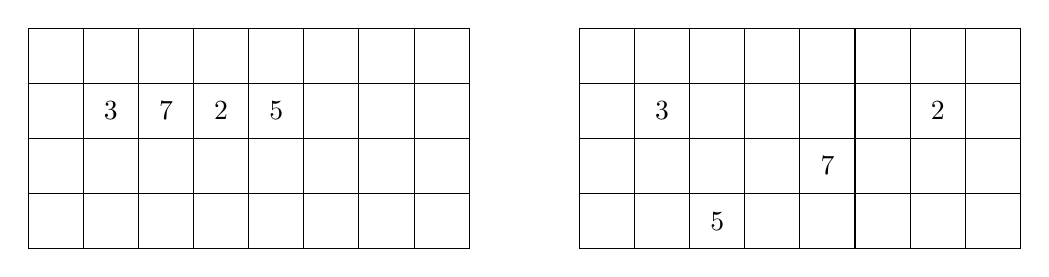
\begin{tikzpicture}[scale=0.7]
\begin{scope}
\draw (0,0) grid (8,4);
\node at (1.5,2.5) {3};
\node at (2.5,2.5) {7};
\node at (3.5,2.5) {2};
\node at (4.5,2.5) {5};
\end{scope}
\begin{scope}[xshift=10cm]
\draw (0,0) grid (8,4);
\node at (1.5,2.5) {3};
\node at (4.5,1.5) {7};
\node at (6.5,2.5) {2};
\node at (2.5,0.5) {5};
\end{scope}
\end{tikzpicture}
\caption{Taulukkolista ja linkitetty lista tietokoneen muistissa.}
\label{fig:taulin}
\end{figure}

Syynä tähän on, että nykyaikaiset tietokoneet
\emph{suosivat} taulukkolistan käyttämistä linkitetyn listan sijaan.
Kuvassa \ref{fig:taulin} näkyy, miten taulukkolista ja linkitetty lista
asettuvat tietokoneen muistissa.
Taulukkolistan alkiot ovat peräkkäin, kun taas linkitetyn
listan alkiot voivat olla eri puolilla muistia sekalaisessa
järjestyksessä.
Nykyaikaisen prosessorin välimuistit ja komentojen ennustus
on toteutettu niin, että ne ovat parhaimmillaan silloin,
kun tieto on tallennettu muistissa peräkkäin -- eli juuri kuten
taulukkolistassa.
Tämä näkyy käytännössä siinä, että taulukkolistan käsittely on selvästi
tehokkaampaa kuin linkitetyn listan käsittely.